\documentclass{article}
% \usepackage[utf8]{inputenc}
\usepackage{titling}
\usepackage{amsmath,amssymb}
\usepackage{siunitx}
\usepackage{graphicx}
\usepackage{subfig}

\makeatletter
\newcommand*{\centerfloat}{%
  \parindent \z@
  \leftskip \z@ \@plus 1fil \@minus \textwidth
  \rightskip\leftskip
  \parfillskip \z@skip}
\makeatother

\title{Applied Reinforcement Learning\\
        \vspace{-0.25cm}
        {\large SS 2019}\\
        \vspace{0.25cm}
        {Project Final Report --- Obstacle Avoidance}}

\author{
  \small Akbar, Uzair\\
  \small \texttt{3697290}
  \and
  \small G\"undogan Alperen\\
  \small \texttt{3694565}
  \and
  \small Ellouze, Rachid \\
  \small \texttt{3671114}
}

\date{July 16, 2019}

\begin{document}
\begin{titlingpage}
    \maketitle
    \begin{abstract}
This report presents our progress for the TUM Applied Reinforcement Learning class project (Summer Semester 2019). We have successfully completed a simple implementation of the Q-learning algorithm for obstacle avoidance using LIDAR ranging data. The agent is tested in a Stage simulator environment and selected preliminary results are presented herein.
    \end{abstract}
    \tableofcontents
\end{titlingpage}
% \section*{Abstract}

\section{Introduction \& Project Objectives}
We start off by quickly reiterating our problem statement and solution objectives. We intend to implement a solution for the obstacle avoidance problem for a turtlebot robot using a LIDAR sensor. The two metrics (which we shall try to quantify in the form of a reward function in section 3.3) to evaluate the quality of our solution are:
\begin{itemize}
\item The turtlebot covers maximum distance within an episode.
\item The turtlebot avoids collisions.
\end{itemize}

\section{Simulation Environment Setup}
\begin{figure}[ht]
 \centering
 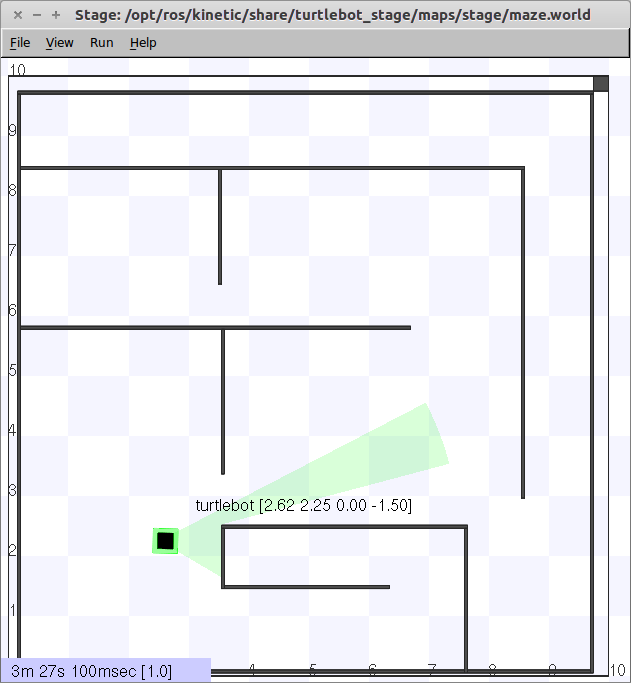
\includegraphics[width=.33\textwidth]{stageSim.png}
  \caption{Turtlebot in the Stage simulator environment.}
  \label{fig:stage}
\end{figure}
As discussed in our project proposal report, we chose to implement our Reinforcement Learning (RL) based obstacle avoidance solution first in a simulation environment, mainly for quick prototyping purposes. We shall later generalize to the real world using prospective approaches as listed in the proposal report. However, this report is primarily concerned with simulation-only implementation of our solution.

We used the Stage simulator to set-up or training environment as shown in Figure \ref{fig:stage}. Because the LIDAR sensor that is provided on the turtlebot does ranging estimates in a horizontal, 2D-plane, it was preferable to use a 2D simulator such as Stage so as to reduce unnecessary computational overhead.

The model of our environment, the reinforcement-agent and the Q-learning algorithm were implemented using the Python programming language. We used the rospy client API to interface our Python scripts with the Robot Operating System (ROS). The main motivation behind the use of Python is ease of implementation.

Upon starting the turtlebot Stage simulator, we run the \texttt{rl\_agent} node$^\ast$, which interacts with the simulator environment. Our RL agent subsequently starts receiving LIDAR ranging data at every time-step (set to $\delta t = 0.14$ sec.) over \ang{360} with a resolution of \ang{1}. This data is pre-processed (details discussed in section 3.1) and is used to model our problem as an MDP to be solved by our RL-agent. The control signals of the RL-agent are published which moves the turtlebot in the simulation accordingly.

% We used the Stage simulator to test our implementation. We had to manipulate the laser sensor to align with actual turtlebot LIDAR sensor i.e. \ang{360} with \ang{1} resolution. The idea is to run the turtlebot stage simulator then run the "rl\_agent" node which interacts with the simulator environment. We used the rospy library for the sake of simplicity e.g. easy to apply RL algorithms. Our RL agent receives the laser data at each simulation time step which is set to $dt = 0.14sec$, filters and discretizes it. Then, RL agent applies an action i.e. chooses linear and angular velocity from the action space and publishes this action to the topic "/cmd\_vel\_mux/input/teleop" to move the base of the turtlebot. If the turtlebot is so close to the wall which in our case the threshold is $0.3m$, the episode is terminated and the turtlebot restarts to move from the same location.

\section{The RL Agent}
We implemented our MDP as described in our project proposal report. However, we restate some of the details here because they have either been changed slightly or were not as clearly communicated in the project proposal report.

\subsection{State Space Definition}
Similar to our proposal, we define the state-space as $\mathcal{S} := \big\{ s\,\big\vert \, s= [\,d^T\:,\,v\,,\,w\,]^T \big\}$, where $d$ is the depth vector observed from the on-board LIDAR sensor. To leverage temporal information, $v$ and $w$ are linear and angular velocities of the robot respectively and are discretized as
\begin{equation*}
  v\in V := \big\{ 0.4, 0.2\,\si{m.s^{-1}}\big\}, \;\;\;w\in W:=\big\{ \frac{\pi}{6}, \frac{\pi}{12}, 0, -\frac{\pi}{12}, -\frac{\pi}{6}\,\si{rad.s^{-1}}\big\}.
\end{equation*}
Similarly, we also discretize $d$ into angular sectors as well as radially (details in section 4), to achieve a final vector of size of $5 \times 6 = 36$ (unless stated otherwise), enumeration over all possible values of which gives $5^6$. Hence, in total, our state space consists of $5^6 * 2 * 5 = 156250$ discrete states.

\subsection{Action Space Definition}
The control space $\mathcal{A}$ shall determine the permissible linear and angular velocities for the turtlebot. We explored two possible discretizations of the action space:
\begin{enumerate}
    \item $\mathcal{A}_1 := \Big\{ a \;\Big\vert\; a = \big(v', w'\big), \;v'\in V, \;w'\in W \Big\}$, where $v'$ and $w'$ are next state linear and angular velocities of the robot respectively. Hence, $\vert \mathcal{A}_1 \vert = 10$. This simply means that the current action determines what the velocity part of the next state should be.
    \item A simpler/smaller action space where $v'$ and $w'$ are ``decoupled,'' --- $\mathcal{A}_2 := \big\{ a\; \big\vert \;a \in \mathcal{A}_1\,,\: v' = v \,\text{or}\,\; w' = w \big\}$, with $\vert \mathcal{A}_2 \vert = 7$. 
\end{enumerate}

\subsection{The Reward Function}
Our task for the turtlebot is for it to go as fast as possible without any collisions. For this, we can employ a simple, action agnostic stage-wise reward function
\begin{equation*}
  r(s) =
  \begin{cases}
    v \cdot \cos(w) \cdot \delta t & \text{if episode running,} \\
    -10 & \text{if collision.}
  \end{cases}
\end{equation*}
The cosine term penalizes meaningless rotation, and $\delta t$ is the time-step for our turtlebot (set to 0.14 s).

\section{Preliminary Results}
\subsection{General Training Configuration}
The following setting should be taken as default in all of our experiments unless stated otherwise for comparitive study purposes.
\begin{itemize}
\item {\bf State Space:} The LIDAR sensor delivers readings over \ang{360} degrees (\ang{1} precision) of range measurements up to 6.5 meters. The original LIDAR space is then $[\ang{0}, \ang{360}) \times [0, 6.5m[$. We have discretized the two dimensions separately. Range values are divided radially into 5 levels --- $[0, 0.5[$, $[0.5, 1[$, $[1, 1.5[$, $[1.5, 2.5[$ and $[2.5, 6.5[$. The intuition behind higher resolution in near-range regions is that it is very critical to select an action when the robot is close to an obstacle. For angles, we limited ourselves to $[\ang{-60}, \ang{60}]$ interval for now, which is divided 6 equal sectors.
\item {\bf Action Space: } Both, linear and angular velocities are not obtained directly from the environment. They are read directly from the previously taken action, as defined by action space $\mathcal{A}_2$. This presents a way to encode the previous states, as the MDP do not allow history dependent policies.
\item {\bf RL Algorithm:} We use simple Q-learning with eligibility traces and $\epsilon$-greedy behaviour policy and enumerate over the states using a look-up table.
\end{itemize}

\subsection{Experiments}
In order to find (or validate) reasonable values for the above mentioned default configurations, we conducted the preliminary following experiments, all of which have been performed 5 times over 250 episodes and the results are aggregated and plotted in Figure 2 as mean and standard-deviation of the cumulative rewards of that respective episode.
\begin{itemize}
\item {\bf State Space:} We compared the default LIDAR discretization strategy with lower radial discretization of only the 3 lower levels and compared the cumulative rewards per episode in Figure 2 Part (a). Similarly, we compared the sector-wise angular discretization with 3 and 10 equal radial segmentation as shown in Figure 2 Part (b).
\item {\bf Action Space: } Both, $\mathcal{A}_1$ and $\mathcal{A}_2$ are compare in Figure 2 Part (d), and, as expected, $\mathcal{A}_2$ outperforms $\mathcal{A}_1$ on at least the rate of learning (the quality of solution for higher epochs remain to be seen).
\item {\bf Eligibility Traces:} For completeness purposes (and more for debugging purposes), we compared the results of eligibility traces implementation with that of no eligibility traces, and as expected got better performance for the former.
\end{itemize}








\begin{figure}[p]
\centerfloat
\begin{tabular}{c c}
\subfloat[Radial resolution of LIDAR readings.]{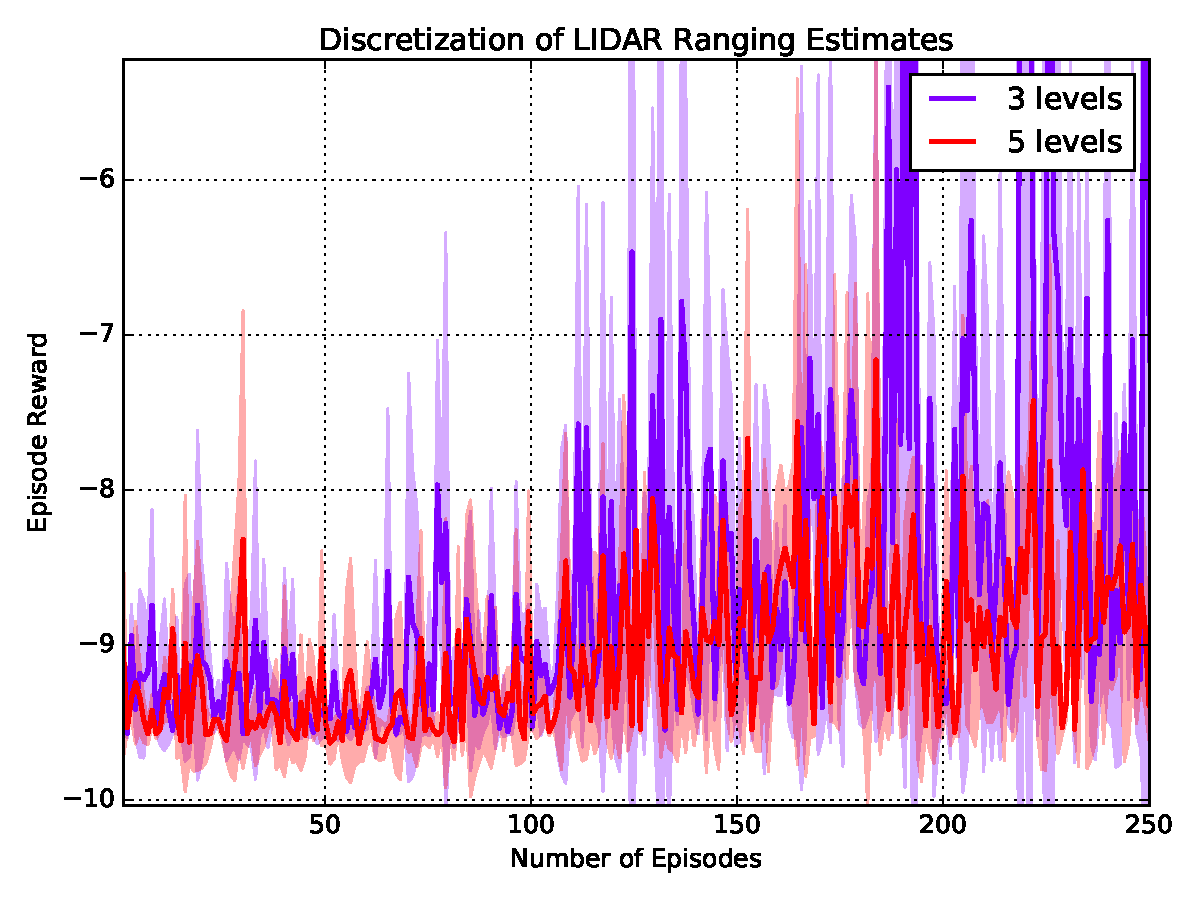
\includegraphics[width=0.49\textwidth]{rangeLevels.pdf}\label{fig:a}}
&
\subfloat[Angular resolution of LIDAR readings.]{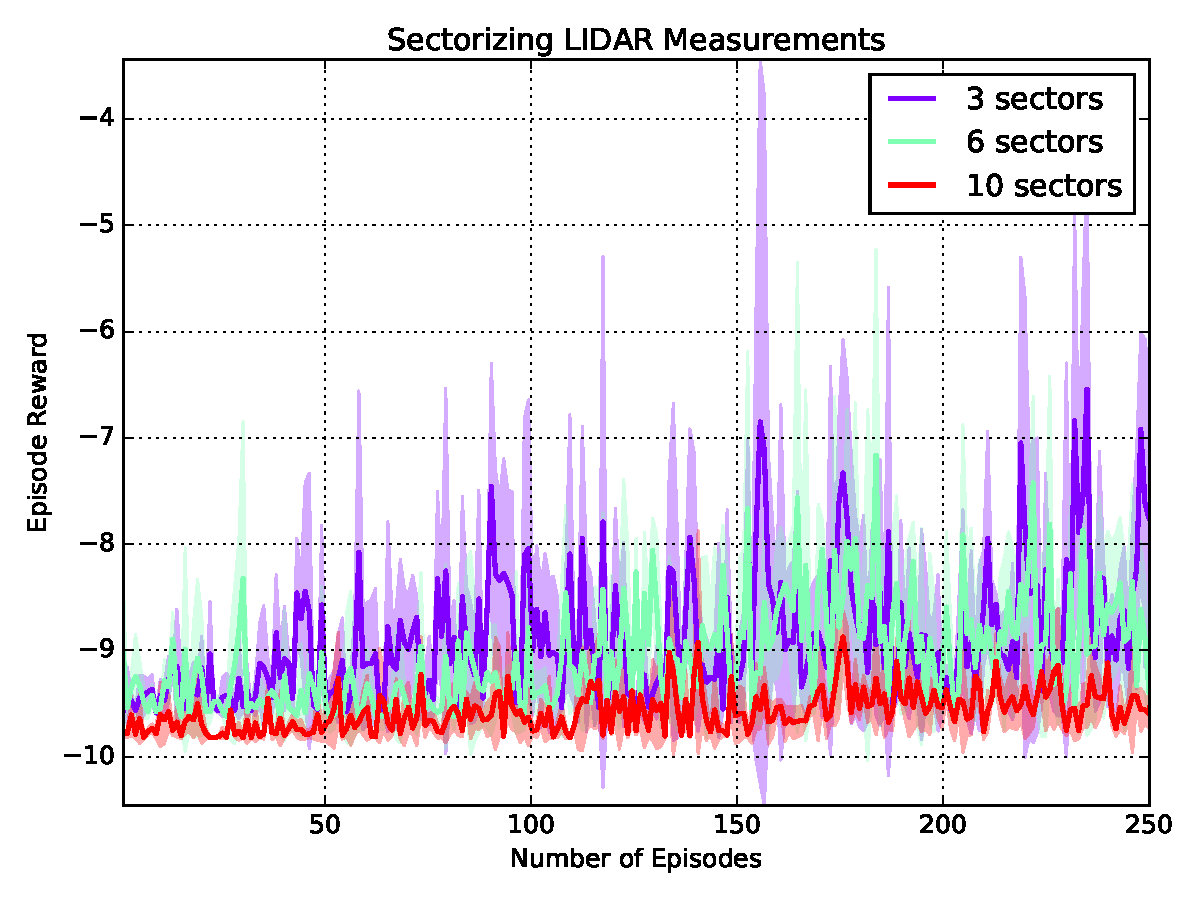
\includegraphics[width=0.49\textwidth]{sectorLevels.pdf}\label{fig:b}}
\\
\subfloat[Eligibility traces vs. no eligibility traces.]{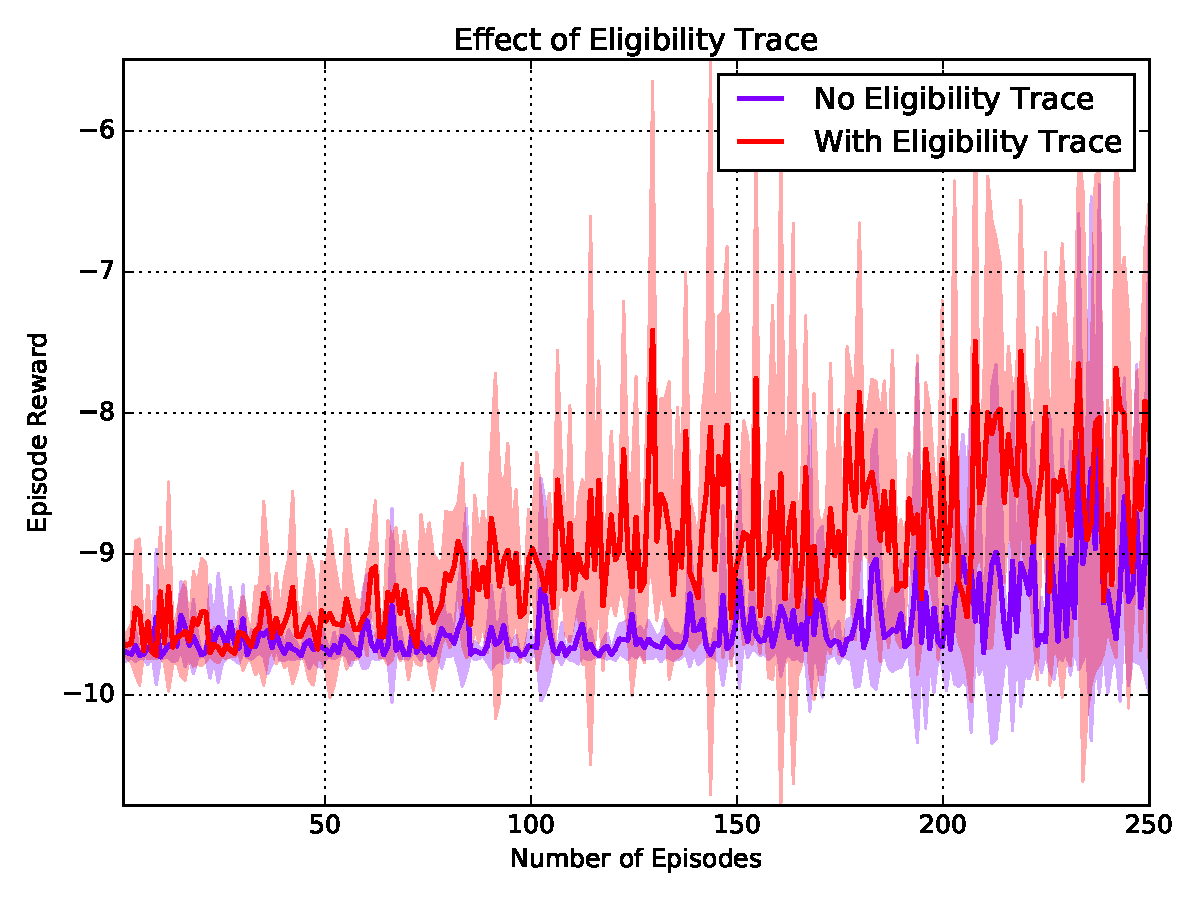
\includegraphics[width=0.49\textwidth]{eligibilityTrace.pdf}\label{fig:c}}
&
\subfloat[Comparing action spaces $\mathcal{A}_1$ \& $\mathcal{A}_2$.]{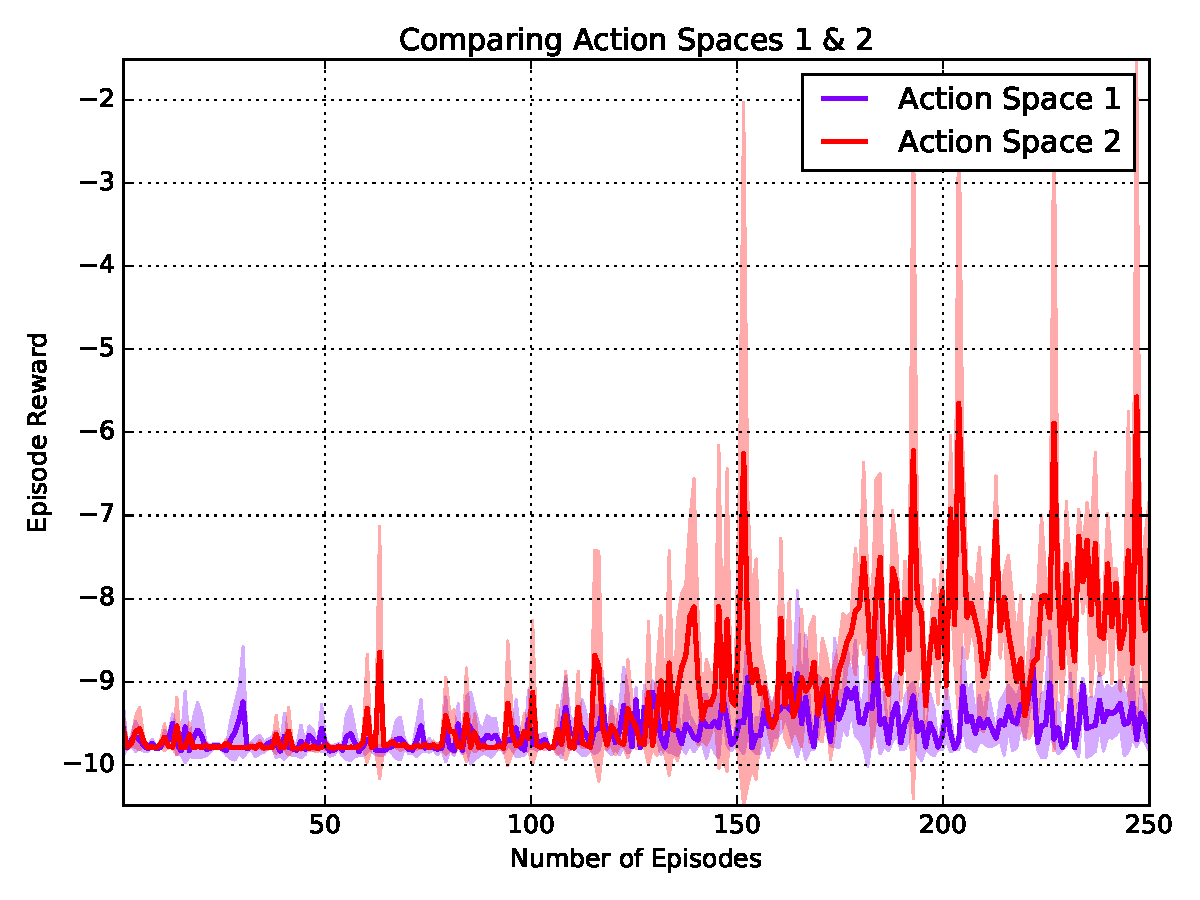
\includegraphics[width=0.49\textwidth]{actionSpace2.pdf}\label{fig:d}}
\end{tabular}
\caption[]{Preliminary results for comparison of different training settings.}
\label{fig:results}
\end{figure}

\section{Future Works}
\begin{itemize}
\item Test the implemented algorithms in real environment and tune the paramters to improve the results.
\item Implement better feature extraction method e.g. autoencoder.
\item Implement SARSA with LVFA on $\epsilon$ - greedy policy. 
\item Implement better action space and reward signals.
\item Implement and compare sof-tmax policy with $\epsilon$-greedy.
\item Determine the final approach and parameters to be used in the real turtlebot.
\end{itemize}
\medskip
% \bibliographystyle{ieeetr}
% \bibliography{references}



\end{document}
